%%
%% PT Slides Template
%% Full-featured template demonstrating all capabilities
%%
%% Author: Pedro Toledo Correa
%% Version: 0.1
%% Date: 2025-10-18
%%

\documentclass{pt-slides}
% Available options:
% - Language: spanish (default), english, portuguese, french
% - Code: nominted (disable minted, use verbatim)
% - Beamer options: aspectratio=169 (default), 12pt (default)

% Document metadata
\title{Título de la Presentación}
\titlesub{Subtítulo Opcional}
\titlesubsub{Sub-subtítulo Opcional}

% Version control
\version{1.0}
\build{auto}  % Use 'auto' for automatic build counting or specify a number
% \watermark{BORRADOR}  % Uncomment to add watermark

% Authors (add as many as needed)
\addauthor{Nombre}{Apellido}{correo@ejemplo.com}{Departamento, Universidad}

% Background image (no logo for this template)
\background{figures/background-default}
% \backgroundcredit{\href{https://upload.wikimedia.org/wikipedia/commons/9/9b/Neckarsulm_-_Scheuerberg_-_Ansicht_von_Westen_im_Oktober_%282%29.jpg}{Roman Eisele, CC BY-SA 4.0, via Wikimedia Commons}}
\backgroundcredit{Roman Eisele, CC BY-SA 4.0, via Wikimedia Commons}

% Optional: Add institutional logo
% \logo{path/to/logo}

% Academic/Class information (optional)
\classcode{IWI-131}
\classname{Programación}
\classsemester{Primer Semestre 2025}

% Institution information (optional)
\department{Departamento de Informática}
\school{Escuela de Ingeniería}
\university{Universidad Técnica Federico Santa María}

% Date
\date{\today}

% TOC Options (customize visibility of table of contents)
\ptshowtoc        % Show TOC at beginning (default: true)
\ptshowsection    % Show section TOC before each section (default: true)
\pthidesubsection % Hide subsection TOC (default: false)
\ptshowlastframe  % Show "Questions?" final slide (default: true)

\begin{document}

% Title and TOC are automatically generated at the beginning

\section{Introducción}

\begin{frame}
    \frametitle{Bienvenida}

    Esta es una plantilla completa que demuestra todas las capacidades de la clase \inlinecode{pt-slides}.

    \vspace{0.5cm}

    \textbf{Características principales:}
    \begin{itemize}
        \item Diseño profesional con imagen de fondo
        \item Generación automática de título y TOC
        \item Gestión avanzada de autores con afiliaciones
        \item Control de versiones en el pie de página
        \item Todas las características del paquete \inlinecode{pt-commons}
    \end{itemize}
\end{frame}

\begin{frame}
    \frametitle{Opciones de la Clase}

    El documento puede configurarse con diferentes opciones:

    \begin{enumerate}
        \item \textbf{Idiomas:} spanish, english, portuguese, french
        \item \textbf{Código:} nominted (desactiva minted)
        \item \textbf{Beamer:} aspectratio, font size, etc.
    \end{enumerate}

    \vspace{0.5cm}

    \begin{highlightbox}
        \textbf{Nota:} La relación de aspecto por defecto es 16:9 y el tamaño de fuente es 12pt.
    \end{highlightbox}
\end{frame}

\section{Formato de Texto}

\begin{frame}
    \frametitle{Estilos Básicos}

    El texto puede ser \textbf{negrita}, \textit{cursiva}, \underline{subrayado}, o \texttt{monoespaciado}.

    \vspace{0.5cm}

    También se puede combinar \textbf{\textit{negrita con cursiva}}.

    \vspace{0.5cm}

    Para código en línea, use: \inlinecode{variable\_name}

    \vspace{0.5cm}

    \begin{block}{Bloque de Ejemplo}
        Los bloques se pueden usar para destacar contenido importante.
    \end{block}
\end{frame}

\begin{frame}
    \frametitle{Listas con Viñetas}

    Las listas tienen espaciado optimizado:

    \begin{itemize}
        \item Primer elemento de nivel uno
        \item Segundo elemento de nivel uno
              \begin{itemize}
                  \item Elemento de nivel dos
                  \item Otro elemento de nivel dos
              \end{itemize}
        \item Tercer elemento de nivel uno
    \end{itemize}
\end{frame}

\begin{frame}
    \frametitle{Listas Numeradas}

    Las listas numeradas tienen formato consistente:

    \begin{enumerate}
        \item Primer paso del procedimiento
        \item Segundo paso del procedimiento
              \begin{enumerate}
                  \item Sub-paso 2.1
                  \item Sub-paso 2.2
              \end{enumerate}
        \item Tercer paso del procedimiento
    \end{enumerate}
\end{frame}

\section{Tablas}

\begin{frame}
    \frametitle{Tablas Básicas}

    La clase utiliza \inlinecode{tabularray} para tablas mejoradas:

    \vspace{0.3cm}

    \begin{table}
        \centering
        \begin{tblr}{colspec={|l|c|c|}}
            \hline
            \tableheader Método & Precisión & Tiempo \\
            \hline
            \hline
            Algoritmo A         & 95\%      & 10s    \\
            \hline
            Algoritmo B         & 97\%      & 15s    \\
            \hline
            Algoritmo C         & 93\%      & 8s     \\
            \hline
        \end{tblr}
        \caption{Comparación de algoritmos}
    \end{table}
\end{frame}

\begin{frame}
    \frametitle{Tablas Avanzadas}

    Tabla con sub-encabezados y celdas personalizadas:

    \vspace{0.3cm}

    \begin{table}
        \centering
        \begin{tblr}{colspec={|l|c|c|c|}, width=0.95\textwidth}
            \hline
            \tableheader
            \tablecellcenter Característica                       & Clase A              & Clase B & Clase C \\
            \hline
            \hline
            \tablesubheader            \tablecellbold Rendimiento & Alto                 & Medio   & Bajo    \\
            \hline
            Velocidad                                             & 100                  & 75      & 50      \\
            \hline
            Memoria                                               & 512 MB               & 256 MB  & 128 MB  \\
            \hline
            \tablecellbold Total                                  & \tablecellbold 100\% & 75\%    & 50\%    \\
            \hline
        \end{tblr}
        \caption{Características de las clases}
    \end{table}
\end{frame}

\section{Figuras}

\begin{frame}
    \frametitle{Inserción de Figuras}

    Las figuras se insertan con comandos estándar:

    \begin{figure}
        \centering
        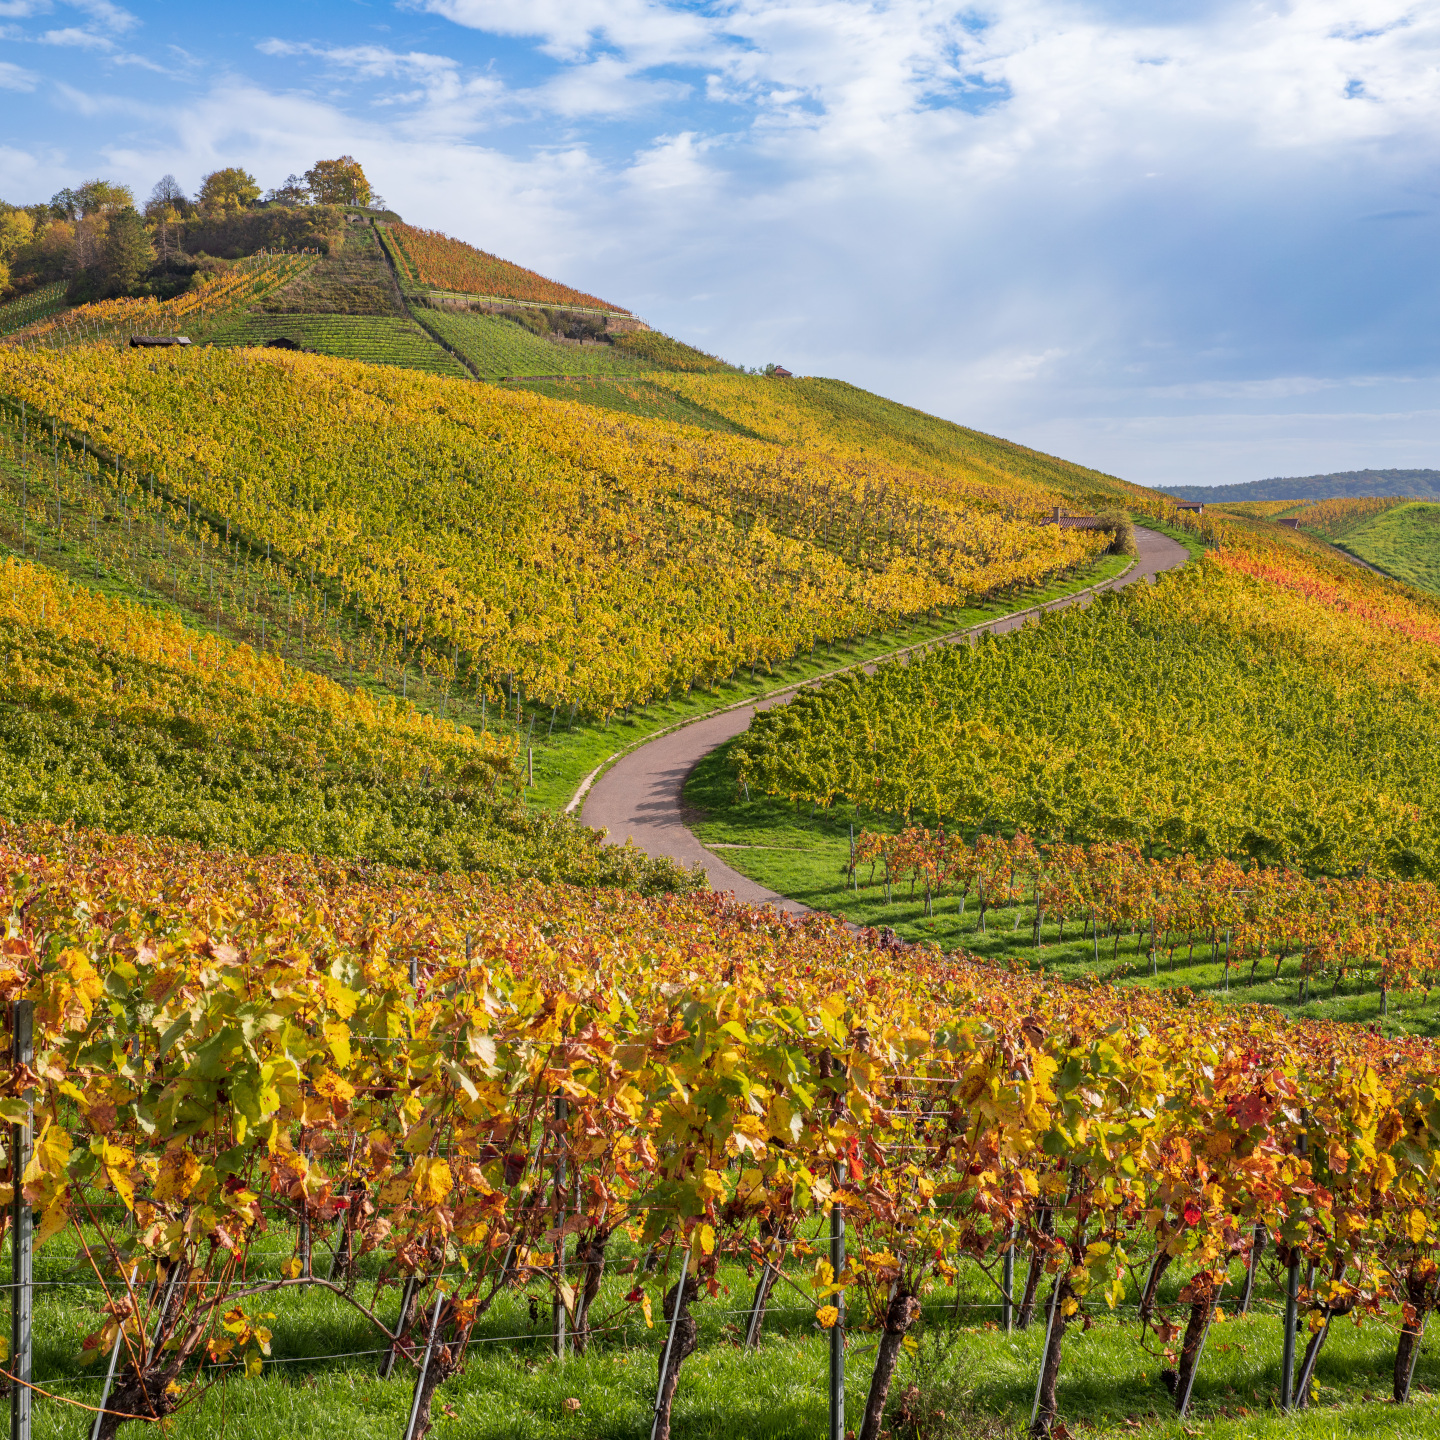
\includegraphics[width=0.5\textwidth]{figures/background-default}
        \caption{Ejemplo de figura}
    \end{figure}
\end{frame}

\begin{frame}
    \frametitle{Figuras Lado a Lado}

    \begin{columns}
        \begin{column}{0.48\textwidth}
            \begin{figure}
                \centering
                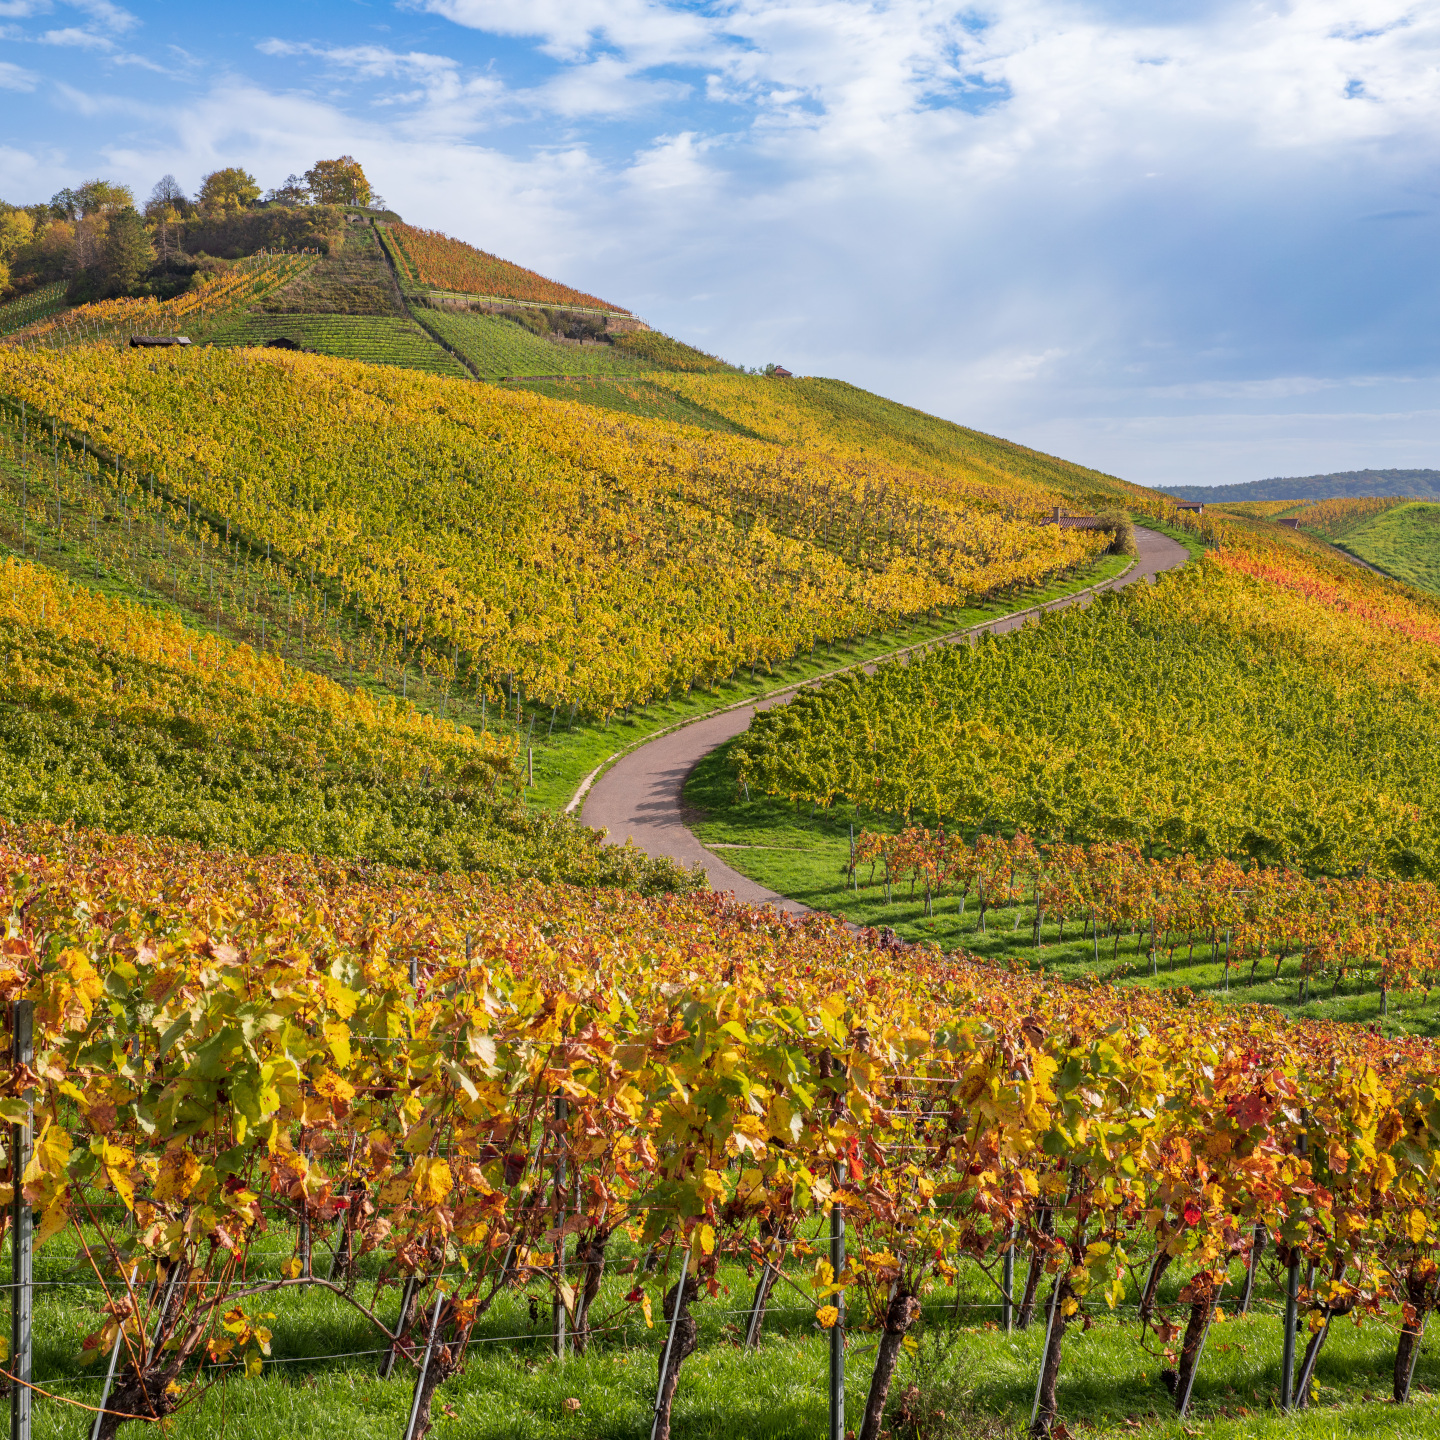
\includegraphics[width=0.8\textwidth]{figures/background-default}
                \caption{Primera figura}
            \end{figure}
        \end{column}
        \begin{column}{0.48\textwidth}
            \begin{figure}
                \centering
                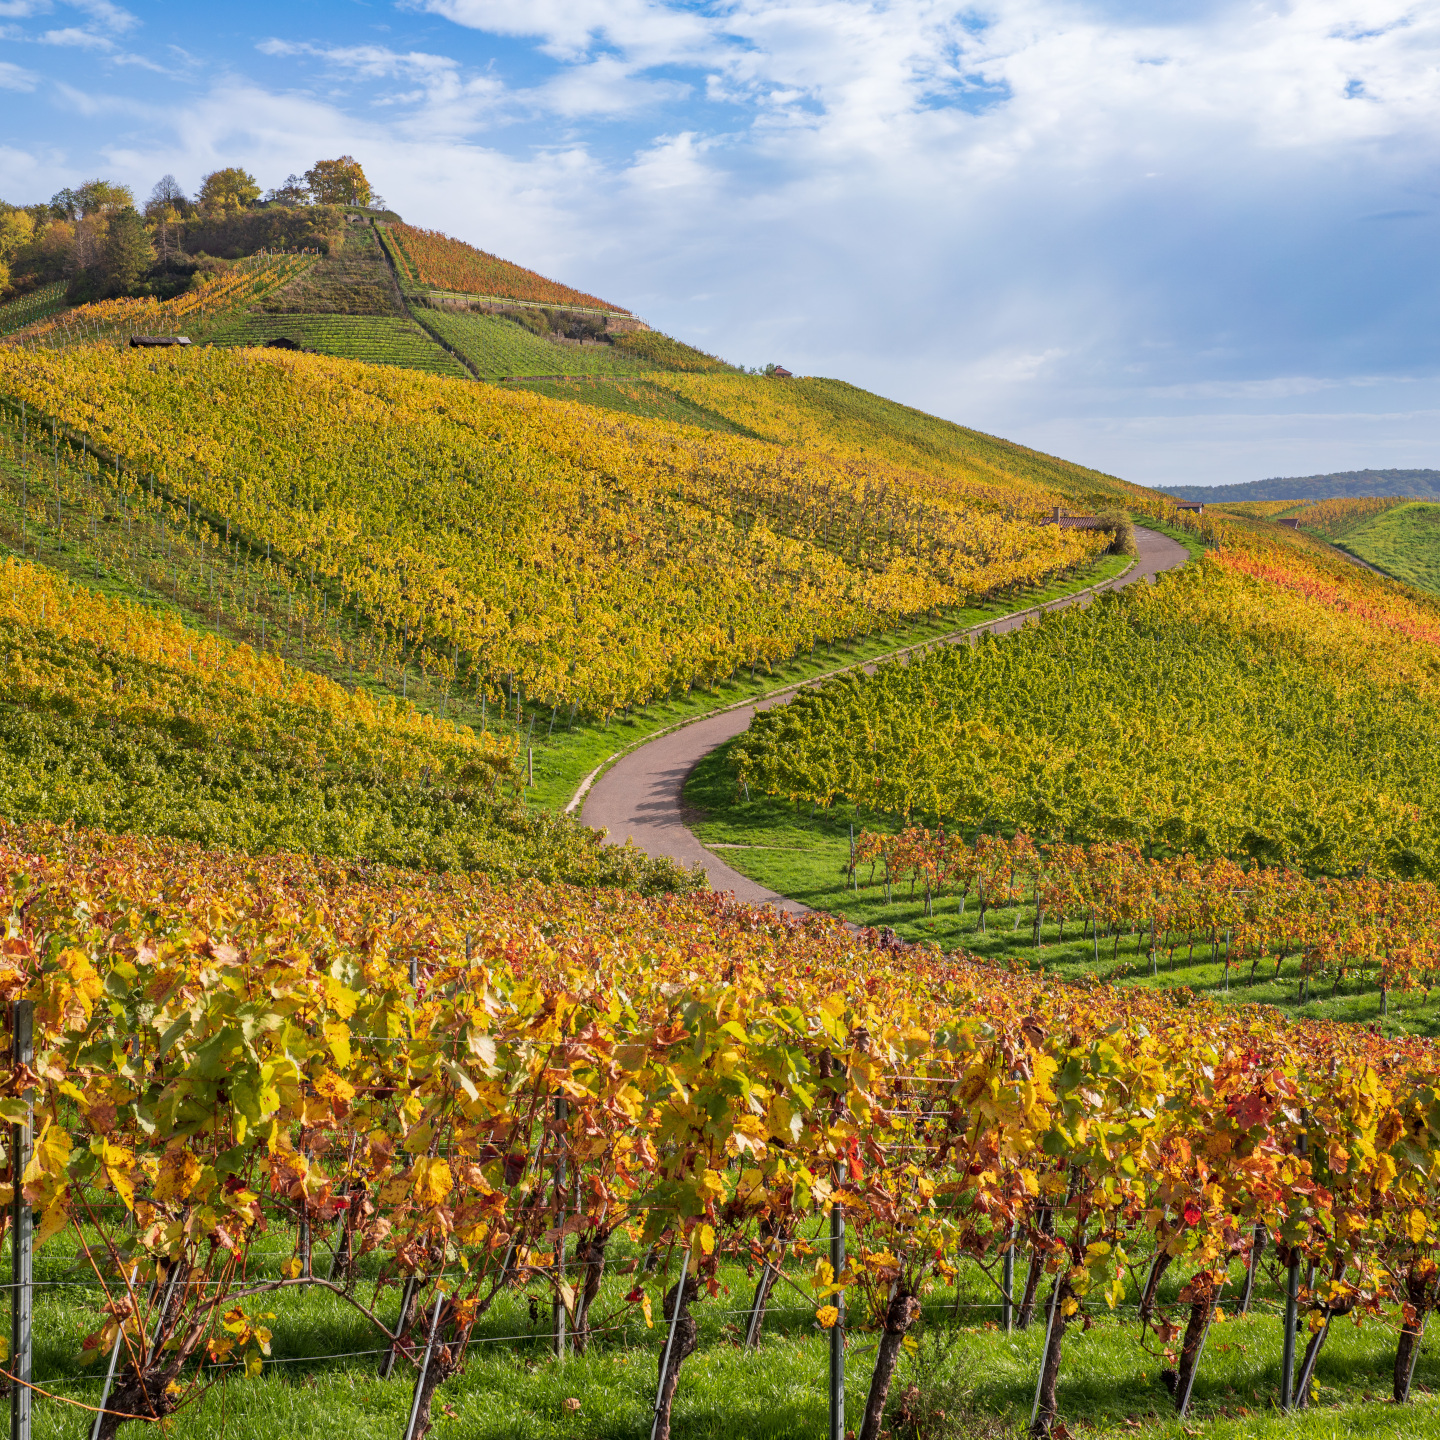
\includegraphics[width=0.8\textwidth]{figures/background-default}
                \caption{Segunda figura}
            \end{figure}
        \end{column}
    \end{columns}
\end{frame}

\section{Código Fuente}

\begin{frame}[fragile]
    \frametitle{Código en Línea}

    Use \inlinecode{\textbackslash{}inlinecode\{\}} para código en línea:

    \vspace{0.5cm}

    Ejemplos:
    \begin{itemize}
        \item Python: \inlinecode{def function():}
        \item C: \inlinecode{int main()}
        \item JavaScript: \inlinecode{const variable = 42;}
    \end{itemize}
\end{frame}

\begin{frame}[fragile]
    \frametitle{Bloques de Código con Minted}

    Con minted habilitado (compile con \inlinecode{-shell-escape}):

    \vspace{0.3cm}

    \begin{minted}[fontsize=\footnotesize]{python}
def fibonacci(n):
    """Calculate Fibonacci number."""
    if n <= 1:
        return n
    return fibonacci(n-1) + fibonacci(n-2)

# Example usage
result = fibonacci(10)
print(f"Fibonacci(10) = {result}")
    \end{minted}
\end{frame}

\begin{frame}[fragile]
    \frametitle{Código para Impresión}

    Use \inlinecode{ptprintcode} para código en blanco y negro:

    \vspace{0.3cm}

    \begin{ptprintcode}{c}
        #include <stdio.h>

        int main() {
                printf("Hello, World!\n");
                return 0;
            }
    \end{ptprintcode}
\end{frame}

\section{Matemáticas}

\begin{frame}
    \frametitle{Ecuaciones en Línea}

    Las ecuaciones en línea se escriben entre \$:

    \vspace{0.5cm}

    La ecuación $E = mc^2$ es una de las más famosas de la física.

    \vspace{0.5cm}

    También podemos escribir: $\int_{0}^{\infty} e^{-x^2} dx = \frac{\sqrt{\pi}}{2}$
\end{frame}

\begin{frame}
    \frametitle{Ecuaciones Numeradas}

    Las ecuaciones se pueden numerar automáticamente:

    \begin{equation}
        \int_{0}^{\infty} e^{-x^2} dx = \frac{\sqrt{\pi}}{2}
    \end{equation}

    \vspace{0.3cm}

    \begin{align}
        f(x)   & = x^2 + 2x + 1 \\
        f'(x)  & = 2x + 2       \\
        f''(x) & = 2
    \end{align}
\end{frame}

\section{Árboles de Archivos}

\begin{frame}[fragile]
    \frametitle{Estructura de Directorios}

    La clase incluye soporte para visualización de estructura de directorios:

    \vspace{0.3cm}

    \begin{ptdirtree}
        \dirtree{%
            .1 \treeiconfirst{proyecto/}.
            .2 \treeicon{src/}.
            .3 \treeicon{main.py}.
            .3 \treeicon{utils.py}.
            .2 \treeicon{docs/}.
            .3 \treeicon{README.md}.
            .2 \treeicon{tests/}.
            .3 \treeicon{test\_main.py}.
            .2 \treeicon{requirements.txt}.
        }%
    \end{ptdirtree}
\end{frame}

\section{Colores}

\begin{frame}
    \frametitle{Paleta de Colores PT}

    La clase proporciona una paleta de colores predefinida:

    \begin{itemize}
        \item \textcolor{ptred}{Rojo PT (ptred)}
        \item \textcolor{ptlightblue}{Azul Claro PT (ptlightblue)}
        \item \textcolor{ptblue}{Azul PT (ptblue)}
        \item \textcolor{ptdarkblue}{Azul Oscuro PT (ptdarkblue)}
        \item \textcolor{ptgreen}{Verde PT (ptgreen)}
        \item \textcolor{ptyellow}{Amarillo PT (ptyellow)}
        \item \textcolor{ptgray}{Gris PT (ptgray)}
    \end{itemize}
\end{frame}

\section{Layouts Especiales}

\begin{frame}
    \frametitle{Columnas}

    \begin{columns}
        \begin{column}{0.48\textwidth}
            \textbf{Columna Izquierda}
            \begin{itemize}
                \item Punto uno
                \item Punto dos
                \item Punto tres
            \end{itemize}
        \end{column}
        \begin{column}{0.48\textwidth}
            \textbf{Columna Derecha}
            \begin{enumerate}
                \item Primer paso
                \item Segundo paso
                \item Tercer paso
            \end{enumerate}
        \end{column}
    \end{columns}
\end{frame}

\begin{frame}
    \frametitle{Caja de Resaltado}

    Use el entorno \inlinecode{highlightbox} para información importante:

    \vspace{0.3cm}

    \begin{highlightbox}
        \textbf{Nota Importante:} Esta es una caja de resaltado que llama la atención sobre información clave. Es útil para advertencias, notas importantes, o conceptos destacados.
    \end{highlightbox}
\end{frame}

\section{Control de TOC}

\begin{frame}
    \frametitle{Opciones de Tabla de Contenidos}

    Puede controlar la visibilidad de TOC con comandos:

    \begin{itemize}
        \item \inlinecode{\textbackslash{}ptshowtoc} - Mostrar TOC inicial
        \item \inlinecode{\textbackslash{}pthidetoc} - Ocultar TOC inicial
        \item \inlinecode{\textbackslash{}ptshowsection} - Mostrar TOC por sección
        \item \inlinecode{\textbackslash{}pthidesection} - Ocultar TOC por sección
        \item \inlinecode{\textbackslash{}ptshowsubsection} - Mostrar TOC por subsección
        \item \inlinecode{\textbackslash{}pthidesubsection} - Ocultar TOC por subsección
        \item \inlinecode{\textbackslash{}ptshowlastframe} - Mostrar slide final
        \item \inlinecode{\textbackslash{}pthidelastframe} - Ocultar slide final
    \end{itemize}
\end{frame}

\section{Compilación}

\begin{frame}[fragile]
    \frametitle{Compilación Estándar}

    Para compilar la presentación:

    \vspace{0.3cm}

    \textbf{Compilación básica:}
    \begin{minted}[fontsize=\footnotesize]{bash}
pdflatex template.tex
    \end{minted}

    \vspace{0.5cm}

    \textbf{Con minted (resaltado de código):}
    \begin{minted}[fontsize=\footnotesize]{bash}
pdflatex -shell-escape template.tex
    \end{minted}
\end{frame}

\section{Conclusión}

\begin{frame}
    \frametitle{Resumen}

    Esta plantilla demuestra todas las capacidades de \inlinecode{pt-slides}:

    \begin{itemize}
        \item Diseño profesional con imagen de fondo
        \item Gestión automática de TOC y navegación
        \item Control de versiones integrado
        \item Soporte completo de pt-commons
        \item Personalización flexible
    \end{itemize}

    \vspace{0.5cm}

    \begin{highlightbox}
        Para más información, consulte el repositorio: \\
        \url{https://github.com/ptoledo-teaching/pt-slides}
    \end{highlightbox}
\end{frame}

% Final slide with "Questions?" is automatically generated

\end{document}
